\section*{S7.3(D)}
\begin{figure}[H]
\centering
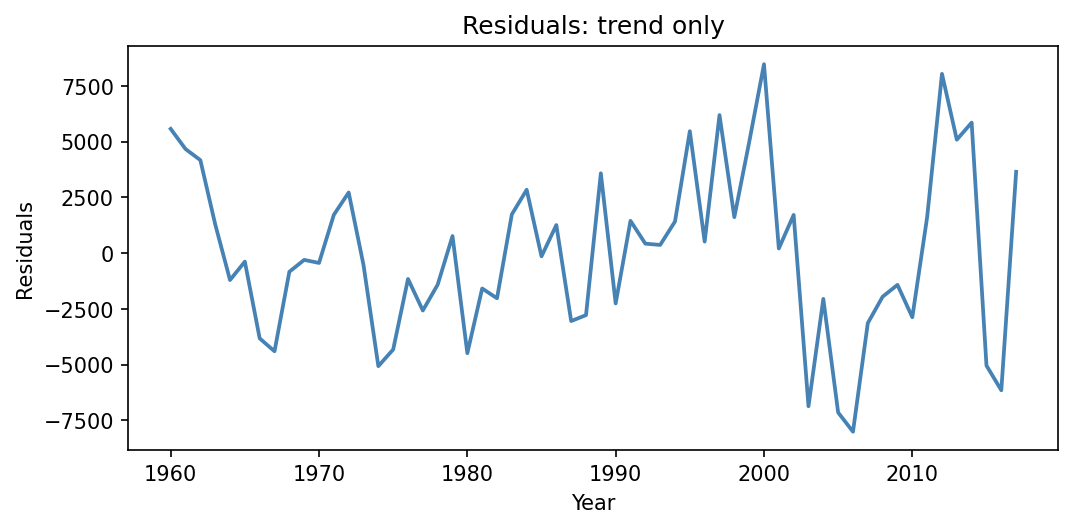
\includegraphics[width=0.95\linewidth]{S7.3D_resid_trend_only.png}
\caption{Residuals from trend-only model}
\end{figure}
\begin{figure}[H]
\centering
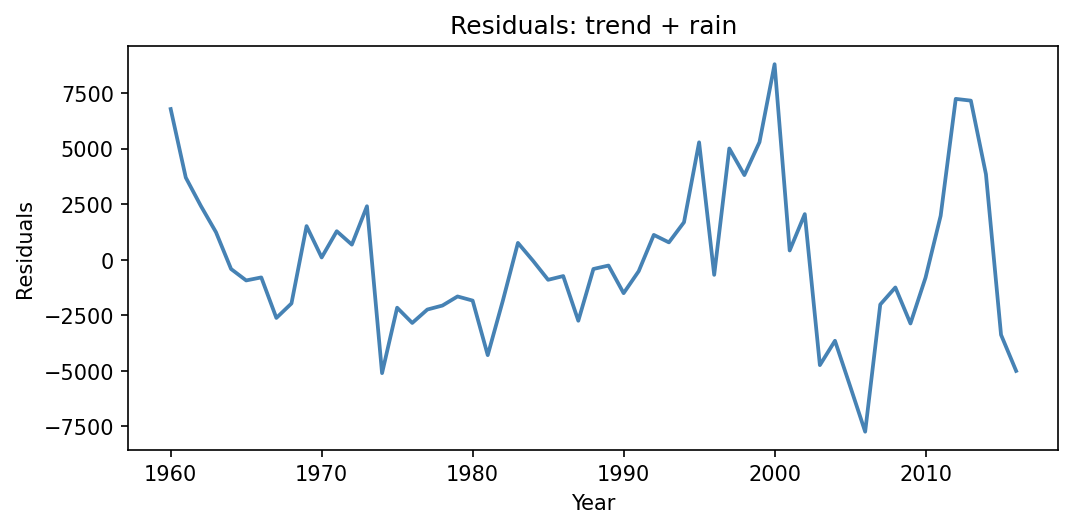
\includegraphics[width=0.95\linewidth]{S7.3D_resid_trend_rain.png}
\caption{Residuals from trend + rain model}
\end{figure}
\begin{figure}[H]
\centering
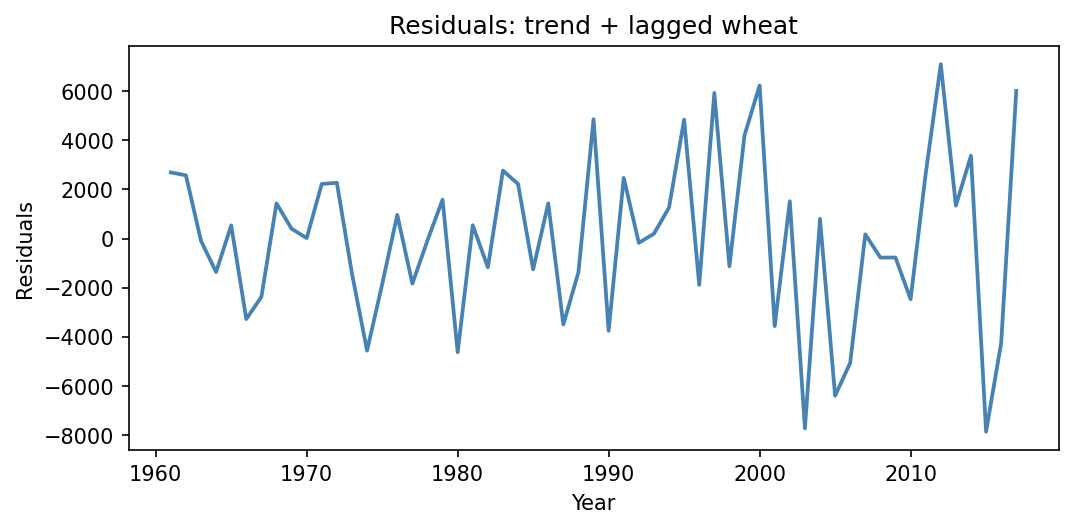
\includegraphics[width=0.95\linewidth]{S7.3D_resid_trend_lag_only.png}
\caption{Residuals from trend + lagged wheat model}
\end{figure}
\begin{figure}[H]
\centering
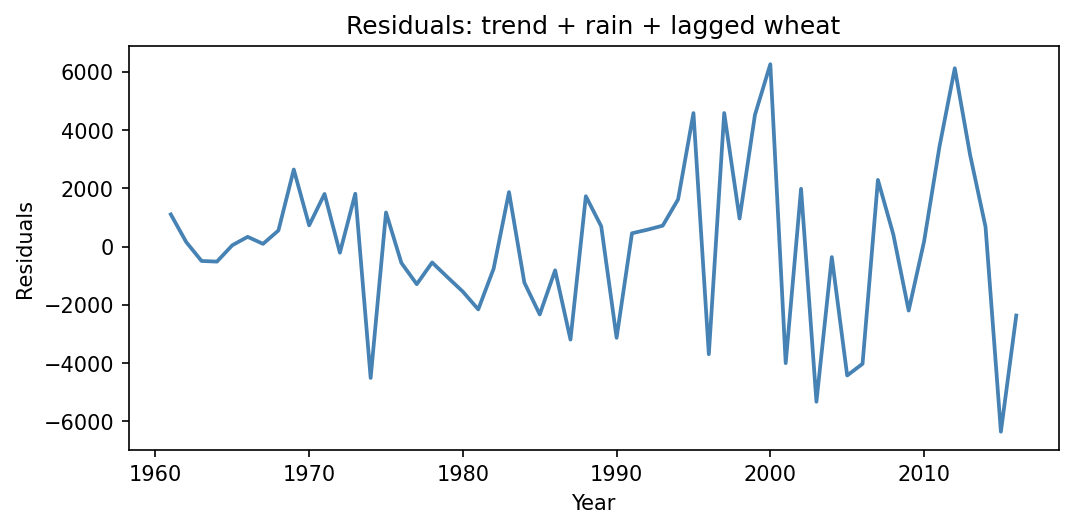
\includegraphics[width=0.95\linewidth]{S7.3D_resid_trend_rain_lag.png}
\caption{Residuals from trend + rain + lagged wheat model}
\end{figure}
Trend-only: $DW=1.093$; Ljung--Box $Q(4)=16.136$ ($p=0.003$). 
Trend + rain: $DW=0.766$; Ljung--Box $Q(4)=27.315$ ($p=0.000$). 
Trend + lagged wheat: $DW=2.035$; Ljung--Box $Q(4)=2.738$ ($p=0.603$). 
Trend + rain + lagged wheat: $DW=1.840$; Ljung--Box $Q(4)=3.665$ ($p=0.453$). 
Interpretation: adding lagged wheat substantially reduces serial correlation relative to trend-only or trend+rain, 
suggesting persistence in output that is not explained by rainfall alone. Rain may help explain levels but does not 
eliminate autocorrelation without a dynamic term.
